\documentclass[12pt]{article}
\usepackage{epsfig}
\textwidth 7.5in                     % page width in inches
\textheight 9.9in                    % page height in inches
\topmargin -90pt                     % to fit on A4
\oddsidemargin -36pt                 % Left hand margin (odd pages)
\evensidemargin -28pt
\baselineskip 0.168in
\setlength{\parindent}{20pt}
%\def\etal{{\it et al. }}
\def\etal{et al.\ }
\newcommand{\msun}{\hbox{M$_{\odot}$}}

\begin{document}

\noindent
\centerline{\bf \textit{Shane Observations with UCSC ASTR 257: Modern Astronomical Techniques}} 
\centerline{\bf PI A.\ Skemer}

\vskip 15pt

\centerline{\bf  Scientific Justification: }

As part of UC Santa Cruz Astronomy's graduate curriculum, Andy Skemer and Xavier Prochaska teach an observing class, which consists of a week-long field trip to Lick Observatory.  The class is required of all first-year graduate students, and ensures that (1) our students will develop a broad range of observational skills at a time when opportunities to develop these skills are becoming more rare, and (2) our students will develop experience with Lick Observatory facilities, which will incentives them to become immediate scientific users.  This class has some parallels to the graduate observing workshop that has been run for many years at Lick Observatory, but the formal course will be more time intensive and will fulfill specific department requirements.

2019 was the first time we offered this class.  It was a huge success, with eleven students completing a class where they used Lick facilities to do astrometry, photometry, spectroscopy, and adaptive optics.  A publicly accessible github account with the class schedule, lectures, observing activities and raw data is available at https://github.com/askemer/ASTR257.  The class was canceled in 2020 due to COVID.

We are planning two observations with the Shane 3-meter.  We will observe edge-on galaxies with the KAST spectrograph to replicate the Vera Rubin experiment, and we will observe Neptune with Shane-AO to make a 3-color image.  We request 3 hours of KAST time for the galaxies observation and 3 hours of AO time for Neptune.  For scheduling reasons, we prefer these observations to take place at the beginning of the night.
\\\\
\textbf{Proposed schedule for ASTR 257}\\
Saturday, 9/18—Arrive and Tour\\
Sunday, 9/19—Observe with Nickel (1st half)\\
Monday, 9/20—Observe with Nickel (1st half)\\
Tuesday, 9/21—Observe with Refractor (1st half)\\
Wednesday, 9/22—Observe with NGS-AO (1st half)\\
Thursday, 9/23—Observe with KAST (1st half)\\
Friday, 9/24—Depart


\newpage

\begin{figure*}[t!]
  \centering
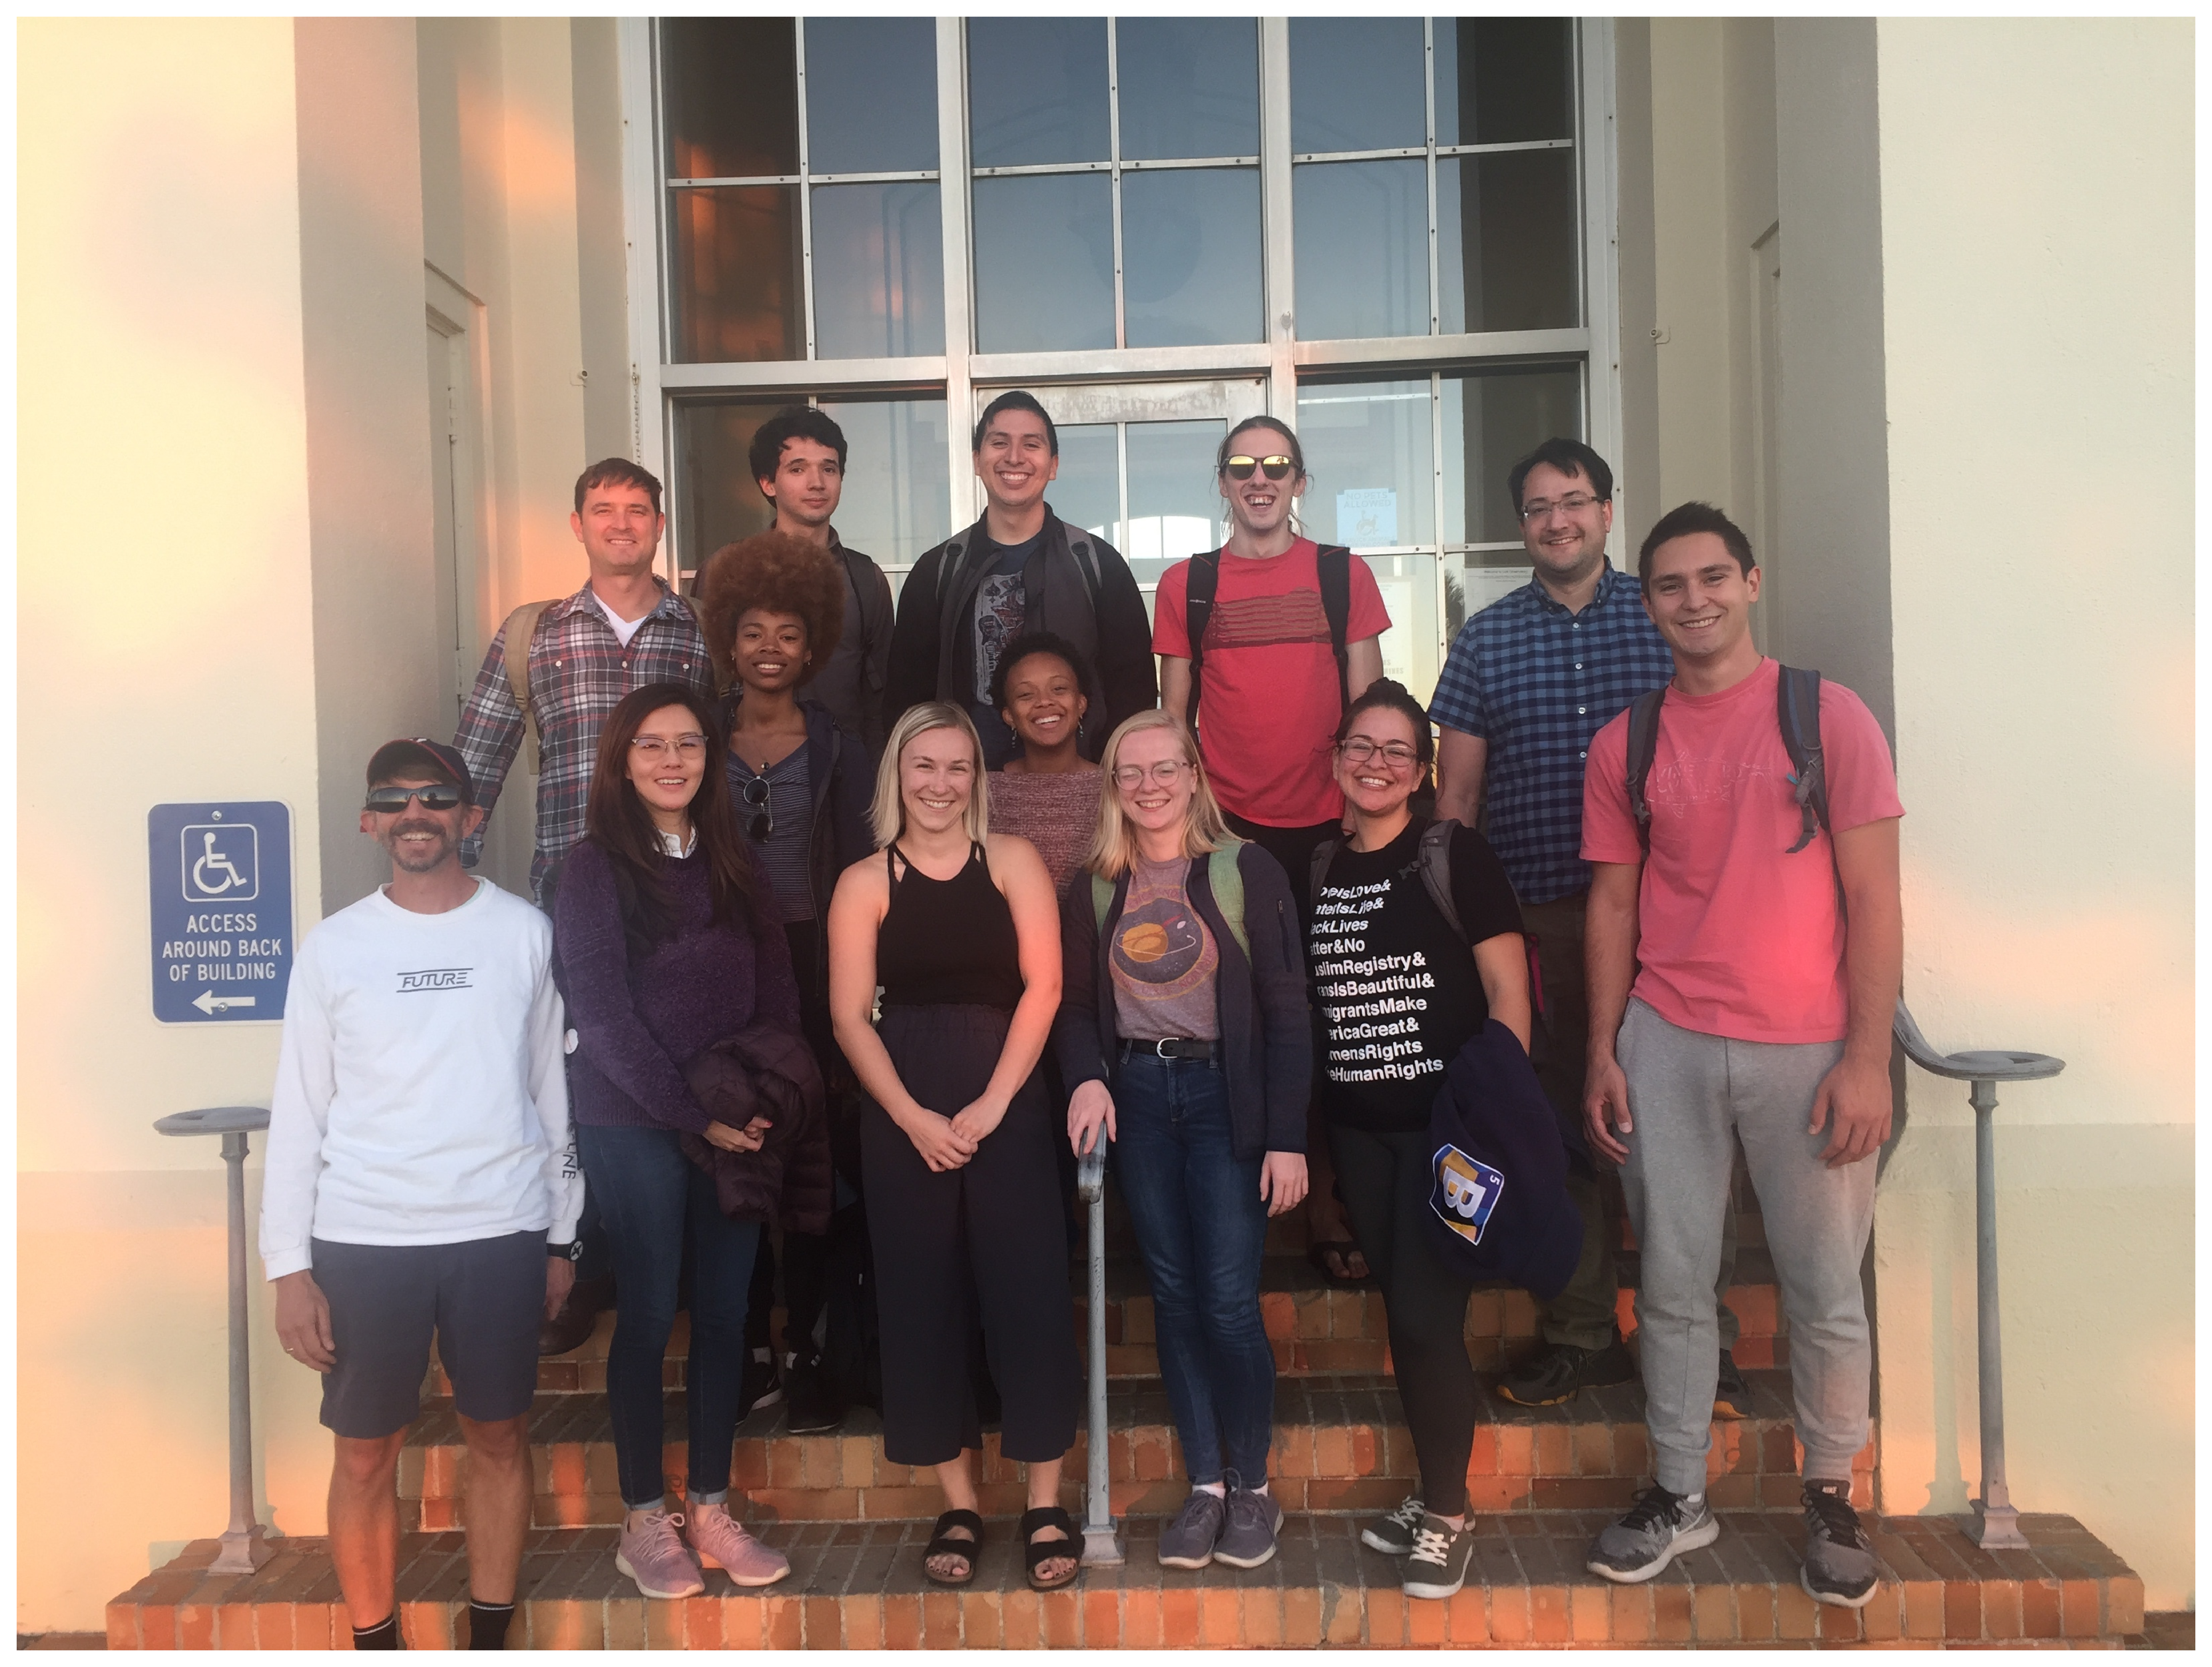
\includegraphics[width=15cm]{ASTR257_2019.pdf}
  \caption{ASTR 257 Class Picture for 2019.  Eleven students participated in the class, nine of whom had never used a professional telescope before.}
\end{figure*}

\begin{figure*}[t!]
  \centering
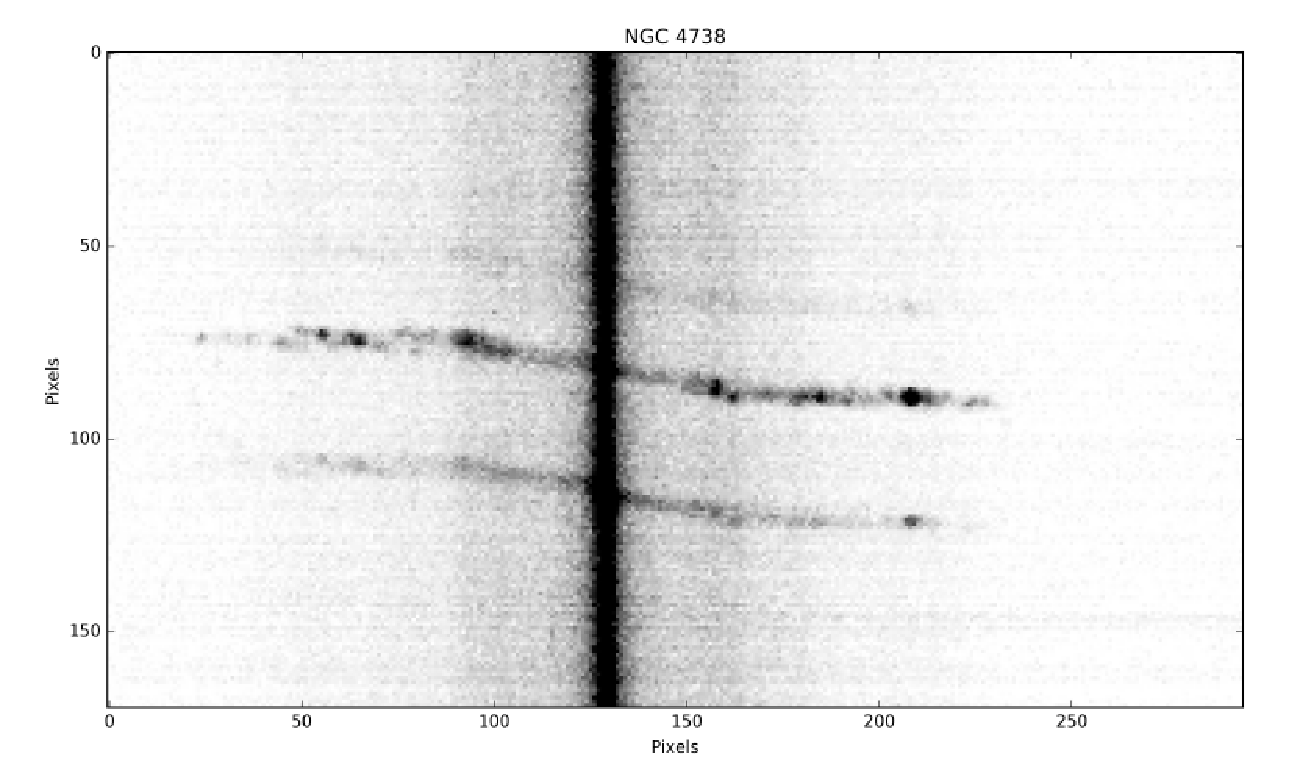
\includegraphics[width=15cm]{fig1.pdf}
  \caption{KAST dispersed image of an edge-on galaxy showing a flat rotation curve.  Image by PHYS 136 student, Zafar Rustamkulov.}
\end{figure*}

\begin{figure*}[t!]
  \centering
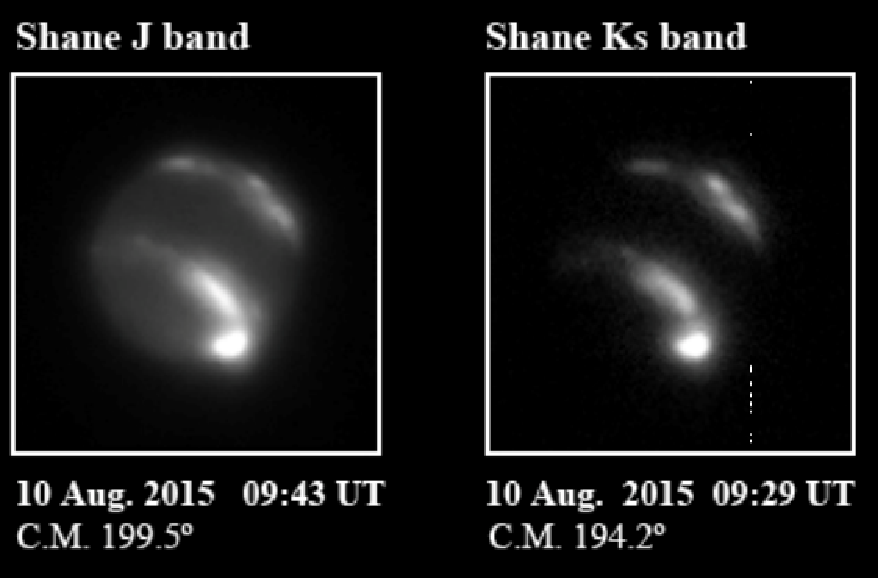
\includegraphics[width=15cm]{fig2.pdf}
  \caption{Shane-AO NGS image of Neptune at multiple wavelengths (Hueso et al. \textit{Icarus}, 2017).}
\end{figure*}

\clearpage

\newpage

\centerline{\bf Technical Remarks}

\noindent
{\bf Targets and Exposures}

\begin{table}[!h]
\begin{tabular}{lllllllllllll}
\hline
Name & instrument \\
\hline
NGC 4738-like objects             & KAST\\
Neptune             & Shane-AO NGS and SHARCS  \\
\hline
\end{tabular}
\end{table}
\noindent
{\bf Supplementary Observations}
None
\\\\
\noindent
{\bf Technical Remarks}
These observations were successful in our 2019 class
\\\\
\noindent
{\bf Path to Science from Observations}
N/A
\\\\
\noindent
{\bf Status of Previous 3-m Programs}
2019--Each ASTR 257 student wrote reports on the KAST spectra and the AO images.  Additionally, we sent the AO images to Ned Molter (UCB) who is doing a monitoring project of Neptune.  Thus, ASTR 257 data will likely end up in a scientific publication.  

\end{document}